\chapter{Monitorização de processos}
\label{cap:trabrelacionado}
O recurso à monitorização do comportamento das aplicações, permite-nos obter dados relevantes sobre os recursos realmente utilizados, de modo a proporcionar-nos um conhecimento mais profundo do seu comportamento em execuções reais e permite igualmente analisar o plano de execução, os métodos mais executados e detectar situações de eventos interessantes.
As informações recolhidas permitem analisar o desempenho ou correcção da aplicação, sequencial ou distribuída, porquanto ao conseguir obter-se dados da utilização do \textit{cpu}, da memória, dos dispositivos de \textit{IO}, interacções, etc, é possível compreender o comportamento dinâmico das aplicações.
Daí ser comum a utilização da monitorização como auxiliar na avaliação e depuração de programas, conseguindo um bom compromisso entre a qualidade dos dados recolhidos e a perturbação das aplicações ~\cite{DuartePhd05}.
 
Na secção \ref{sect:instrumentation_overview} é apresentada a forma de efectuar a monitorização, distinguindo entre os diferentes modos de obtenção da informação.
Na secção \ref{sub:network_monitoring} é apresentada a monitorização de rede, onde se centra o foco deste trabalho, como um caso especifico da monitorização, são discutidos alguns dos problemas inerentes a esta monitorização, bem como algumas formas de os mitigar.
É igualmente apresentado o \textit{Packet Capture} (\textit{PCap}), a sua arquitectura e partes relevantes da sua implementação, bem como alguns modos que permitem melhorias no desempenho da rede e da monitorização.

Como a monitorização não é apenas exclusiva da rede, na secção \ref{sect:instrumentacao_casos_linux} são apresentadas ferramentas e mecanismos de monitorização do núcleo.
Estas ferramentas permitem não só instrumentar o código do núcleo, mas também analisar o código de aplicações em nível utilizador.

Como um dos problemas da monitorização é a obtenção da informação relevante, na secção \ref{sect:kernel_user_comm} são apresentados mecanismos de transferência de dados e, sistemas de comunicação entre o núcleo e o nível utilizador, para compreender se existem mecanismos alternativos que possam melhorar o desempenho da monitorização de rede.

Na secção \ref{sect:outras_abordagens} são apresentados exemplos de ferramentas de monitorização de rede com base em informação de processos de nível utilizador.

Por último, na secção \ref{sec:segundo:conclusion} apresenta-se uma conclusão referente aos mecanismos de monitorização e obtenção de informação.

\section{Formas de monitorização}\label{sect:instrumentation_overview}

Os dados relativos ao comportamento das aplicações, obtidos de diferentes fontes, são normalmente coligidos e posteriormente analisados por ferramentas especializadas.
Existem diferentes formas de coligir, visualizar e até interactuar com os monitores, cada uma com as suas especificidades e capacidades próprias.
Algumas são desenvolvidas para objectivos específicos.
Tendo em vista o conhecimento geral das capacidades de cada uma, podemos analisar estes sistemas de variados pontos de vista.

\paragraph*{}
Se considerarmos, por exemplo, quanto à análise e visualização face ao instante da execução da aplicação alvo, podemos dividir os sistemas em:
 
\subparagraph*{Online -}
Enquanto decorre a monitorização da aplicação é possível observar os dados que são recolhidos pelo monitor.
Como os eventos estão a ser recolhidos e visualizados em simultâneo, apenas podemos observar a história até ao momento, mas temos uma baixa latência entre os acontecimentos e a sua observação.

\subparagraph*{Offline ou \textit{Post-Mortem} - }

A história do programa é analisada após este se ter completado, daí a designação \textit{Post-Mortem}.
Este método permite-nos analisar integralmente a sua história e correlacioná-la.
Permite análises mais completas e computacionalmente mais exigentes.

\paragraph*{}

Se a monitorização necessitar de interactividade do utilizador, é possível defini-la de duas formas:

\subparagraph*{Activa - }

Por iniciativa explícita do utilizador, é possível inquirir o sistema de monitorização sobre o estado da computação, ou mesmo alterá-la.
Este método, por vezes descrito como \textit{computacional steering}, é a forma com maior interactividade, uma vez que permite ir analisando e modificando os parâmetros da monitorização ou mesmo da aplicação.

\subparagraph*{Passiva - }
Esta forma de monitorização é especialmente utilizada em ambientes onde é relevante a obtenção de um conjunto fixo de dados e, apenas no final, nos debruçarmos sobre a sua análise.
Esta forma é designada por passiva, pois o utilizador não tem intervenção na forma como os dados estão a ser obtidos, o que reduz a perturbação no sistema.
Quanto muito a sua acção acontece antes da execução, para configuração da informação a recolher.

\paragraph*{}
A própria instrumentação da aplicação pode ser de dois tipos: a estática e a dinâmica, cada uma com características próprias:

\subparagraph*{Estática - }

Na instrumentação estática o código de instrumentação é definido em tempo de compilação ou utilizando bibliotecas próprias para o efeito, como a utilização da função \textit{assert}, que define os pontos a serem monitorizados.
Durante a execução não podem ser adicionados ou removidos pontos de análise.

\subparagraph*{Dinâmica - }

Em contraste com a instrumentação estática está a dinâmica.
É mais complexa que a estática e permite a inserção e remoção dos pontos a serem monitorizados.
Caracteriza-se pela ausência do ciclo $introduzir ponto\rightarrow compilar programa\rightarrow executar\rightarrow remover ponto$ de instrumentação.
A utilização de pontos de instrumentação dinâmica, pode ajudar a reduzir o grau de perturbação, uma vez que apenas são definidos os que se desejam observar.
Tal pode ser efectuado no início ou durante a sua execução, criando, alterando e destruindo os pontos de observação sobre os recursos monitorizados.


\subparagraph*{
%Recolha de dados
}
A recolha de dados provenientes da monitorização é uma das componentes mais sensíveis, relativamente ao grau de perturbação da monitorização.
Em geral as informações recolhidas da monitorização são inicialmente armazenados em memória central e posteriormente em memória persistente.
Esta transferência de memória central para disco em geral deve-se a uma acção explícita do utilizador, ou então, a algum evento indicador da necessidade de guardar os dados, de forma a que novos dados possam ser armazenados em memória, uma vez que os \textit{buffers}, em memória, geralmente têm dimensão fixa.

\subparagraph*{
%Grau de perturbação
}
Existe claro a preocupação de que o sistema a ser monitorizado, tenha um baixo grau de perturbação, pois esta pode levar à alteração dos resultados obtidos e mesmo a comportamentos erráticos da aplicação (especialmente perante execuções concorrentes).
Por este motivo, diversas abordagens foram criadas, para reduzir o impacto da monitorização num sistema em produção.
Uma destas abordagens traduz-se na utilização de instruções especializadas, de que alguns processadores dispõem para \textit{debug}, de modo a utilizar os recursos que mais se adequem à monitorização.
Estes métodos, nem sempre são utilizados, devido à sua dependência da arquitectura, o que dificulta a sua portabilidade.
Com vista a minimizar a perturbação, alguns sistemas de monitorização utilizam uma técnica de amostragem, que permite obter indicações sobre o estado da computação a cada intervalo de tempo.
Esta técnica, em oposição à criação de um traço de execução, permite obter dados sobre os recursos apenas por amostra, limitando à partida a perturbação, enquanto que na criação de um traço de execução, é possível obter a totalidade dos eventos de forma a criar uma história completa, conduzindo a uma grande sobrecarga do sistema perante uma elevada taxa de eventos.

\paragraph*{
}
No entanto, obter dados oriundos da monitorização pode revelar-se insuficiente, se não dispusermos de uma ferramenta onde estes possam ser tratados, de modo a obtermos análises mais completas relacionado-os com os detalhes de funcionamento da aplicação monitorizada.
No entanto estas análises não serão o foco deste trabalho.

\section{Monitorização de Rede}\label{sub:network_monitoring}

As ferramentas de monitorização de rede são, em geral, baseadas na captura de pacotes de forma passiva.
Estas capturam os pacotes que fluem através da interface de rede, para posterior análise ao tráfego, que pode incidir sobre a largura de banda utilizada, principais protocolos, eventuais problemas de segurança, etc.

A monitorização das interacções dos processos com o exterior, pode ser efectuada de diferentes formas, de que se apresentam duas:
A primeira utiliza bibliotecas instrumentadas que obtêm os dados quando estes chegam (ou saem) da aplicação, sendo que a segunda forma recorre a mecanismos genéricos do núcleo, para a monitorização de rede.
Relativamente à primeira, é necessário conhecer o código da aplicação, ou das suas bibliotecas e instrumentá-lo, obtendo-se apenas os dados referentes à aplicação.
Este processo é específico de cada aplicação e pode ver o seu uso limitado por questões de segurança do sistema.
No que à segunda forma se refere, a monitorização é efectuada de forma genérica, não sendo intrusiva para as aplicações, necessitando apenas de efectuar separadamente a monitorização do processo e da rede.

\subparagraph*{Dinamismo das aplicações - }
As aplicações são dinâmicas quanto às interacções via rede (por exemplo criando e destruindo canais de comunicação).
Este dinamismo acarreta algumas dificuldades, ao monitorizar as interacções dos vários fluxos de execução dos processos.

\subparagraph*{Formas de reduzir o volume de dados utilizando filtros - }
A utilização de filtros na captura do tráfego de rede é uma forma eficiente de apenas se obterem os dados relevantes, com vista à satisfação dos nossos objectivos e, são particularmente importantes, quando o volume de dados que circula na rede é extremamente elevado.
Tendo em vista a eficiência, estes filtros são implementados no núcleo do sistema de operação, baseando-se em regras simples, que podem ser combinadas para contemplar situações mais complexas.

\subparagraph*{Dificuldade de criação e alteração de filtros - }
Os filtros actualmente suportados para capturar pacotes no \textit{Linux}, são definidos \textit{a priori}, não existindo forma eficiente de os alterar dinamicamente, uma vez que a captura tem de ser interrompida a fim de ser criado um novo filtro e posteriormente aplicado, procedendo-se em seguida à retoma da captura dos pacotes, de acordo com as novas regras.

\subparagraph*{Filtros complexos - }
Para aumentar o desempenho da captura de pacotes, os filtros são aplicados o mais cedo possível, ou seja, logo na interface de rede.
Face a esta situação, o tipo de filtros que se podem aplicar têm de ser simples, baseados apenas nos metadados do pacote.
Quando os filtros são demasiado complexos, a componente de filtragem do núcleo tem de transferir o pacote para o monitor em nível utilizador, de modo a poder aplicar o filtro.

\subparagraph*{Técnicas para o aumento de desempenho}

Diferentes técnicas têm vindo a ser desenvolvidas para aumentar o desempenho da monitorização das interfaces de rede.
Como já referido, o aumento da sobrecarga é muito penalizante, daí que esta deva ser mantida bastante reduzida, o que contribuirá para aumentar o desempenho da captura.

Actualmente a utilização de máquinas equipadas com processadores \textit{multi-core} é uma realidade, deste modo a sua utilização permite ultrapassar algumas dificuldades sentidas na captura de pacotes.
Se os processadores \textit{multi-core} atenderem em paralelo as diversas interrupções, originadas pelo envio ou recepção de pacotes, o desempenho da rede é passível de ser aumentado.
No entanto, revela-se difícil atingir este paralelismo para todas as interfaces de rede, pois nem todas estão preparadas para beneficiar de arquitecturas com múltiplos \textit{cores}.

\section{Biblioteca \textit{PCap} e \textit{Linux Socket Filtering}}\label{sect:LibPcap}

A monitorização de rede existente em muitos dos sistemas tipo \textit{Unix} e mesmo no \textit{Windows} permite capturar os pacotes de rede logo que estes chegam ao controlador de rede.
Assim, a biblioteca \textit{PCap}\cite{LibPcap} permite às ferramentas de monitorização de rede fazerem uso deste mecanismo.
Uma das principais características desta biblioteca, é a sua \textit{API} de alto nível para a captura de pacotes, que é igual em todas as plataformas.

A monitorização de rede realizada pelas ferramentas que utilizam a biblioteca \textit{PCap}, é efectuada de modo passivo, adequando as suas análises aos pacotes capturados, de modo \textit{online} ou \textit{offline}.
Esta monitorização é não intrusiva para o código das aplicações e, dependendo do modo como é efectuada, pode ter algum impacto no desempenho destas ou no do sistema.

Para filtrar os pacotes indesejados a biblioteca \textit{PCap} utiliza filtros baseados no \textit{Berkeley Packet Filtering} (\textit{BPF}), normalmente implementados no núcleo de sistema, de modo a que a monitorização se torne mais eficiente e menos intrusiva.
Assim, a interactividade apresentada é, em geral, ao nível da alteração dos filtros para a captura.

Em seguida é apresentada a arquitectura da biblioteca \textit{PCap} e o seu suporte no \textit{Linux}, cuja implementação de filtros toma o nome de \textit{Linux Socket Filtering}.

\subsection {Arquitectura}
\label{sect:architecture_libpcap}
A arquitectura do \textit{Packet Capture} (\textit{PCap}) divide-se em duas partes: a biblioteca em nível utilizador, e a implementação do \textit{Linux Socket Filtering} no núcleo de sistema, como é visível na figura \ref{fig:pcap_architecture}.
Como o anteriormente referido, a bibilioteca em nível utilizador é constituída por uma \textit{API} homogénea, que oferece às ferramentas de monitorização de rede um mecanismo para efectuar as suas análises ao tráfego.
As funções auxiliares da biblioteca efectuam chamadas ao sistema de modo a interagirem com o mecanismo de monitorização de rede do \textit{Linux}, \textit{Linux Socket Filtering}.

\begin{figure}[htbp]
       \centering
       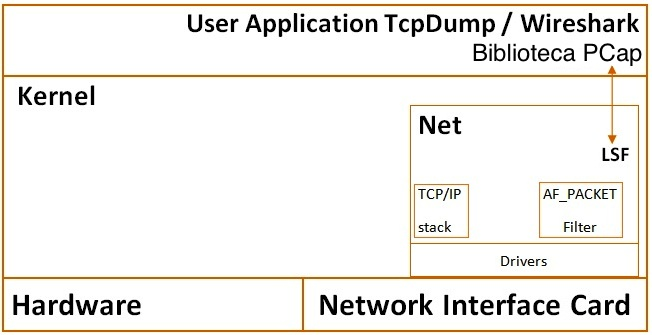
\includegraphics[scale=0.7]{tcpdump.jpg}
%       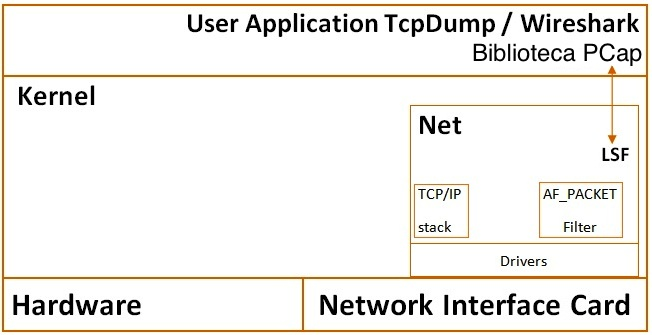
\includegraphics[scale=0.5]{tcpdump}
       \caption{Arquitectura da biblioteca \textit{PCap} e do \textit{LSF}}
      \label{fig:pcap_architecture}
\end{figure}

\subsection{Biblioteca}

A biblioteca em nível utilizador, ao ter uma \textit{API} homogénea entre plataformas, permite aos programadores desenvolverem mais rapidamente ferramentas de monitorização de rede multiplataforma, sendo utilizada pela generalidade das ferramentas de monitorização de rede, tais como o \textit{TcpDump}, o \textit{Wireshark}, o \textit{Snort}, etc.
Esta biblioteca como é multiplataforma, permite ao programador utilizá-la nos principais sistemas de operação, dado que a \textit{API} da biblioteca \textit{PCap} é transparante relativamente à implementação, esta sim, específica a cada plataforma.
Existem implementações da biblioteca \textit{PCap} para \textit{Linux}, \textit{MS-Windows}, \textit{FreeBSD}, etc.

No \textit{Linux} para cada utilização da biblioteca \textit{PCap} é criado um \textit{socket} da família \textit{AF\_PACKET}.
Este tipo de \textit{socket} permite comunicar directamente com a interface de rede e possibilita a captura dos pacotes que nela circulam, para uso do processo monitor.
Para além da captura, devido à comunicação directa com as interfaces, permite a activação e desactivação de propriedades destas.
Uma destas propriedades é o modo promiscuo, geralmente utilizado para efectuar a captura de pacotes, que não pertencem às comunicações da máquina que efectua a monitorização.
Apesar desta funcionalidade ser amplamente utilizada para a monitorização da rede, para o âmbito desta dissertação é totalmente desnecessária, dado que os pacotes a serem recolhidos para análise, são os pertencentes a processos da máquina.

Um dos parâmetros necessários à monitorização, é a interface sobre a qual irá ser efectuada.
Existe um modo especial, o \textit{any}, de modo a monitorizar todas as interfaces simultâneamente.

Como o atrás referido, quando o número de dados da monitorização é elevado e nem todos os dados capturados são relevantes para as análises, estes podem ser filtrados, o que permite minimizar a sobrecarga ao ignorar de imediato os pacotes não relevantes.
A implementação da biblioteca permite efectuar diversas formas de filtragem, quer em nível utilizador, para filtros mais complexos, quer no núcleo com filtros apenas baseados nos metadados dos pacotes.
Se a filtragem for efectuada exclusivamente em nível utilizador, é necessário pedir ao núcleo do sistema de operação, que todos os pacotes sejam capturados.

A ferramenta que utiliza a biblioteca, especifica um filtro utilizando para tal as instruções pertencentes à biblioteca \textit{PCap}.
Se o filtro for demasiado complexo e não possa ser aplicado no núcleo (como seja quando o \textit{SO} em causa não suporte a funcionalidade requerida), será automaticamente aplicado em nível utilizador, perdendo-se algum desempenho.
Antes da introdução do novo filtro no canal de rede, este tem de ser objecto de drenagem\footnote{signfica garantir que todos os pacotes em trânsito no canal da pilha de rede no \textit{SO} são tratados e entregues, para que a nova captura possa entrar em funcionamento.}, para receber apenas os pacotes de acordo com o novo filtro.
Esta filtragem, evita a captura de pacotes irrelevantes para a análise e permite que aqueles que não são visíveis às aplicações, devido à \textit{firewall} do \textit{Linux}, possam também ser capturados e analisados pelas ferramentas de monitorização de rede.
A função \textit{pcap\_compile}, presente na biblioteca, irá traduzir e optimizar o filtro para o conjunto de instruções do \textit{LSF} (ou o equivalente presente no \textit{SO}), sendo posteriormente aplicado no núcleo através da função \textit{setfilter}.
Esta função utiliza a chamada ao sistema \textit{setsockopt}, passando como argumentos o canal e o filtro a ser executado, para que este passe a ser avaliado para cada pacote recebido ou enviado através da interface de rede.
Caso o número de \textit{bytes} dos pacotes sejam superiores ao indicado no filtro, o pacote é cortado até ao tamanho indicado neste.
É possível obter estatísticas, relacionadas com a captura e filtragem de pacotes, através de \textit{ioctls} efectuadas sobre o canal de recepção da monitorização.

A arquitectura de rede do núcleo de sistema \textit{Linux}, utiliza \textit{socket buffers}, que contêm os dados referentes às diferentes camadas da pilha de rede \textit{TCP/IP}.
Esta estrutura dispõe de toda a informação sobre o pacote, não só o \textit{payload} recebido pelas aplicações, como também os metadados, sendo utilizada na implementação dos filtros no \textit{LSF}.

As ferramentas que utilizam esta biblioteca, não necessitam de conhecer estes mecanismos internos, sendo-lhes facultada a \textit{API} que lhes permite abstrair das especificidades da arquitectura onde estão a executar.


\subsection{Linux Socket Filtering}

O \textit{Linux Socket Filtering} (\textit{LSF}), pertence à arquitectura de rede do núcleo do \textit{Linux}.
Este componente permite que sejam efectuadas monitorizações ao tráfego que circula nas interfaces de rede, de modo não intrusivo.
Como o anteriormente referido, o \textit{LSF} utiliza um \textit{socket} da família \textit{AF\_PACKET} que comunica directamente com o controlador da interface de rede, possibilitando a captura dos diversos pacotes ainda antes destes puderem ser filtrados pela \textit{firewall}, presente no núcleo de sistema.

O \textit{LSF} é derivado do \textit{Berkeley Packet Filtering} (\textit{BPF}) que é o \textit{standard} de \textit{de facto} para a criação de filtros destinados à captura de pacotes de rede, no núcleo de sistema.
Este sistema de captura e filtragem permite aos administradores, definir e afectar filtros ao \textit{socket} da família \textit{AF\_PACKET}, afecto às interfaces onde a captura deve ser realizada.
A linguagem simples utilizada para a criação dos filtros no \textit{PCap} é traduzida para o \textit{Instruction Set}, definido no \textit{BPF}.
Este \textit{Instruction Set} utiliza operadores lógicos de forma a combinar as regras definidas nos filtros, criando-se apenas um filtro a ser aplicado aos pacotes~\cite{Mccanne92thebsd}.
Este filtro é como um programa que irá ser executado, passo a passo, sobre cada pacote, recebido ou enviado, através de uma máquina virtual desenhada para o efeito no \textit{LSF}.
No retorno da execução deste programa / filtro, é indicado se o pacote deve, ou não ser capturado.
Caso seja, é duplicado e, a cópia continua o seu percurso, pelo sistema de monitorização, até ao monitor em nível utilizador, que em geral é uma ferramenta que utiliza a biblioteca \textit{PCap}.

Na versão actual do núcleo \textit{Linux} (2.6.39), o \textit{socket} \textit{AF\_PACKET} pode utilizar um sistema de partilha de \textit{buffer} (\textit{MMAP}), com o espaço de utilizador.
Neste caso, cabe à ferramenta monitora definir explicitamente que deseja utilizar este modo de captura e, de modo a atingir este objectivo, solicita ao núcleo uma região de memória partilhada, sendo esta, posteriormente, indicada como argumento na configuração do \textit{socket}.

\subsection{Limitações e optimizações}
Apesar da \textit{API} da biblioteca \textit{PCap} existir em diferentes plataformas, o desempenho desta pode variar para cada caso.
Quando existe pouco tráfego de rede as diferenças são pouco notórias, mas logo que este se intensifica, estas acentuam-se bastante, como demonstra o estudo~\cite{Deri2004}.

Diversas razões podem levar à limitação de desempenho por parte da aplicação monitora, sendo que uma destas é a sobrecarga exercida pela necessidade de copiar dados e trocar de contexto entre nível utilizador e o núcleo.
Dependendo de cada implementação e das análises a serem efectuadas, pode ser interessante e vantajoso desligar o modo permiscuo da interface de rede a monitorizar.
Assim, caso este modo esteja desligado, um menor número de pacotes serão processados e transferidos para o monitor, o que reduzirá significativamente a sobrecarga exercida.
Outros mecanismos em especial para a implementação no \textit{Linux}, podem influenciar o desempenho deste sistema, como a seguir se apresenta.
 
\paragraph*{PACKET\_MMAP}

Para diminuir o número de cópias de dados, entre o núcleo e o processo monitor em nível utilizador, foi utilizada a técnica de partilha de um espaço em memória.

Com base nesta técnica de \textit{MMAP}, foi criado o \textit{PACKET\_MMAP}, disponível a partir da versão 1.0.0 da biblioteca \textit{PCap}.
Este módulo permite algumas melhorias em termos de desempenho, face à anterior versão 0.9.8 da biblioteca \textit{PCap}, visto que o número de cópias de dados dos pacotes foi reduzida.

Esta técnica consiste na utilização de um bloco de memória pertencente ao processo monitor, de modo a que não seja necessário voltar a transferir cada pacote capturado do núcleo para a ferramenta.
Este novo método tem de ser acompanhado por contadores/índices de acesso à memória, dado que, esta zona de memória é acedida como um \textit{buffer} circular.
Apesar de melhorar significativamente o número de cópias de dados, como os blocos de memória para a introdução dos pacotes é efectuada de modo estático, existe apenas um número fixo de pacotes que podem ser mantidos.
Deste modo, se o ritmo de escrita dos pacotes na zona de memória for superior ao ritmo de leitura pela ferramenta, podem existir perdas de pacotes, devido à inexistência de espaço para guardar os novos, enquanto os anteriores não forem consumidos.

Para além destas modificações no \textit{PACKET\_MMAP}, o núcleo \textit{Linux} na sua versão 2.6, permite e aconselha a utilização da nova \textit{API} de rede (\textit{NAPI}), apresentada na secção \ref{sub:napi}.


%Se as interfaces de rede suportarem um mecanismo de mitigação de interrupções, é possível obter melhores resultados, conforme \cite{Deri2004}.


\paragraph*{PF\_RING}

Este é um novo módulo para o núcleo \textit{Linux}, criado com base em duas técnicas \textit{mmap} e \textit{ring\_buffers}.

Este módulo difere na abordagem utilizada no \textit{PACKET\_MMAP}, porquanto nesta a memória é mapeada entre a ferramenta e o controlador da interface, enquanto que no \textit{PACKET\_MMAP} aquela é mapeada entre a ferramenta e um \textit{buffer} interno ao núcleo do sistema, mas externo ao controlador da interface.
Esta abordagem permite que os dados fiquem disponíveis para a aplicação directamente, verificando-se a inexistência de cópia dos dados do \textit{buffer} do controlador, para o \textit{buffer} partilhado entre a ferramenta e o núcleo\cite{PFRING}.
 
\paragraph*{PF\_RING com DNA (Direct NIC Access)}
Baseando-se na técnica anteriormente descrita, de utilizar um \textit{buffer} partilhado entre a ferramenta de monitorização e o controlador, assiste-se a uma evolução desta técnica, ao permitir que a interface de rede partilhe um \textit{buffer} com a ferramenta de monitorização, possibilitando que os pacotes passem directamente para esta~\cite{IntroPF_RIDNADirecNICAcces}.
Esta partilha é efectuada utilizando \textit{mmap}, \textit{ring\_buffers} e \textit{DMA} (\textit{Direct Memory Access}).
Para ser utilizada esta técnica, é necessário que a interface de rede, permita a utilização de memória partilhada e \textit{DMA}.

\paragraph*{}

Diversos esforços no sentido de aumentar o desempenho da captura de pacotes têm sido efectuados.
Relativamente ao \textit{software}, são conhecidos esforços na utilização de técnicas de partilha de \textit{buffers}, como o \textit{mmap}, de modo a reduzir o número de cópias de dados entre as aplicações e o núcleo de sistema.
Igualmente no \textit{hardware}, tem-se assistido a uma evolução, no sentido de reduzir as interrupções efectuadas ao \textit{cpu}, adicionando nas interfaces de rede processadores dedicados a certas funcionalidades presentes no núcleo, de modo a libertá-lo da execução de tarefas, designadamente de monitorização, de colocação de estampilha temporal, de reagrupar segmentos, filtragem de pacotes, etc.
Além das funcionalidades já referidas, têm sido igualmente adicionadas multiplas filas de espera, para que estas possam tirar partido das arquitecturas de multiplos \textit{cores} e das memórias \textit{cache} residentes nestes processadores.


%\paragraph{Captura com \textit{dns} activo}
%
%Como já referido, a biblioteca \textit{PCap} é utilizada por diversas ferramentas de análise ao trafego de rede.
%Uma destas ferramentas é o \textit{TcpDump}, tem sido desenvolvida a par com a biblioteca \textit{PCap} .
%
%
%A biblioteca \textit{PCap}
%\textit{TcpDump} com parametro n de \textit{dns} para obter os nomes de dominios sempre que possivel
%
%\paragraph{Captura especificando tamanho máximo de 65535 para pacotes}
%
%MTU de 1500 ethernet


\subsection{Optimizações na Estrutura de Rede}
\label{sub:napi}
Com a utilização de redes a 100 ou 1000 \textit{Mbps} o número de interrupções efectuadas, por unidade de tempo, é muito elevado.
Esta situação implica, que para cada pacote transferido entre o \textit{buffer} da interface de rede e a memória central, seja necessário uma interrupção ao \textit{cpu}.
Quando a utilização de rede é baixa, este modo de atendimento não comporta uma elevada sobrecarga no sistema, todavia a partir de um determinado valor, o número de atendimentos de interrupções é tão alto que torna quase impraticável a realização de trabalho.

Foi criada uma nova \textit{API} (\textit{NAPI}) de atendimento de interrupções do processador, oriundos das interfaces de rede, com o objectivo de aumentar o desempenho da utilização de redes de elevado débito.
Esta nova \textit{API}, permite desligar a atenção do processador a novas interrupções, oriundas da interface de rede, diferindo-as durante um certo período de tempo.
Este tempo é definido, de forma a que não se verifiquem situações de elevada latência na chegada dos pacotes às aplicações.

Actualmente, a arquitectura de rede está balanceada de forma a mudar o modo de atendimento de interrupções para \textit{NAPI}, caso existam demasiadas interrupções por unidade de tempo~\cite{administrator:napi}.

Utilizando esta nova \textit{API}, é possível explorar um escalonamento mais eficiente das interrupções, em situações de intensa actividade da interface de rede e do processador.
O \textit{NAPI}, apenas pode ser aplicado nos caso em que os controladores das interfaces de rede estejam preparados para utilizar alguma forma de mitigação da interrupção, caso contrário esta \textit{API} não pode ser utilizada.

Através desta nova \textit{API}, é possível diminuir o número de trocas de contexto, entre o controlador da interface e o núcleo de sistema.
Sempre que o \textit{cpu} atende uma sequência de interrupções de rede, obtém um maior número de dados, que combinado com um sistema de memória partilhada aumenta substancialmente o desempenho.

\paragraph*{Sistemas \textit{multi-core} e multi-processador}

Com o aparecimento de sistemas \textit{multi-core} e \textit{multi-processador} a que a generalidade do público tem acesso, a paralelização de código ou a forma de tirar partido destas arquitecturas, que permitem um melhor aproveitamento dos recursos, assumem uma particular importância.
De modo a tirar partido das arquitecturas \textit{multi-core} no próprio núcleo do sistema, é necessário que o controlador e interfaces de rede, os \textit{buffers}, e os controladores de \textit{DMA}, sejam modificados de forma a conhecerem esta arquitectura.
É pois, determinante um esforço conjunto envolvendo todas estas componentes, com vista à obtenção do máximo rendimento destas arquitecturas\cite{Deri:2010}.



\section{Sistemas de monitorização no núcleo do \textit{Linux}}\label{sect:instrumentacao_casos_linux}

A monitorização do núcleo é uma das melhores formas de conhecer não só, como os recursos da máquina são partilhados entre o núcleo e os processos, como também efectuar análises de desempenho e correcção dos diversos componentes do núcleo.
Assim nesta secção são apresentadas ferramentas e mecanismos de monitorização presentes no núcleo.

A utilização dos sistemas de monitorização ao nível do núcleo, permitem também efectuar a monitorização genérica dos processos, de forma não intrusiva para as aplicações.
Ao efectuar a monitorização no núcleo, a sobrecarga imposta ao sistema pode ser menor que em nível utilizador, por ser possível recolher apenas as informações presentes no próprio núcleo que sejam relevantes, evitando a recolha e posterior tratamento dos elementos não relevantes.

Neste documento constam apenas mecanismos e ferramentas de monitorização dinâmicas, pois apenas estas são as desejadas para a criação de um mecanismo de monitorização de rede orientada ao processo.
De entre os mecanismos e ferramentas de monitorização dinâmica analisadas é possível agrupá-las em duas categorias: com base em eventos pré-definidos e com base em instrumentação dinâmica.
Na categoria instrumentação dinâmica existem dois mecanismos relevantes: o \textit{KProbes} e o \textit{Linux Kernel Stace Tracer}, enquanto que para os eventos pré-definidos foram verificados o \textit{Linux Trace Toolkit} e o \textit{OProfile}.
Estas quatro ferramentas são apresentados em seguida considerando as suas categorias:

\subsection{Eventos pré-definidos}

Nesta categoria encontram-se duas ferramentas o \textit{Linux Trace Toolkit} e o \textit{OProfile}.
Em cada uma destas ferramentas a monitorização é efectuada sobre pontos previamente definidos, não permitindo a adição de novos pontos de monitorização.
Cada um destas ferramentas analisa todo o sistema, sendo a filtragem extra dos eventos efectuada em nível utilizador.
%\todo{ver}
%Como os eventos detectados através destas ferramentas geram um mapa de execução, a utilização de apenas alguns eventos pré-definidos não é limitativa de uma ferramenta.

\subsubsection{Linux Trace ToolKit}\label{cap:linux_trace_toolkit_overview}

% O Linux Trace Toolkit é uma ferramenta de ``tracing''
% Utiliza o Klog com repositorio da informação obtida do kernel.
% Nesta versão a comunicação entre o kernel e aplicação em user space é efectuada utilizando o relayfs.
% O RelayFs é um sistema de ficheiros para comunicação entre o código dentro e fora do núcleo de operação.
%A utilização desta ferramenta em sistemas de tempo real é um bom indicador da sua performance.

O \textit{Linux Trace ToolKit} (\textit{LTT}) é uma das ferramentas mais utilizadas para efectuar traços de execução do núcleo \textit{Linux}.
Esta ferramenta foi criada no final da década de 1990, sendo posteriormente substituida em 2005 pelo \textit{Linux Trace ToolKit new generation}, (\textit{LTTng}), projecto derivado do \textit{LTT}.
O \textit{LTT} é constituído por quatro componentes: o \textit{Kernel Patch}, o \textit{Kernel Module} o \textit{Trace Daemon} e o \textit{Data Decoder} conforme consta na figura \ref{fig:ltt_arch}.
É através do \textit{Trace Daemon} que o utilizador pode comunicar com o sistema de monitorização.
%Os dados recolhidos têm diversos valores tais como o nome da função, o tempo, e o identificador do processador, pelo menos estes atributos de modo a conseguir construir os traço de execução.
O \textit{LTT} e o \textit{LTTng} são ferramentas de monitorização dinâmica que efectuam um traço de execução.
O \textit{Linux Trace Toolkit New Generation}, utiliza os mecanismos \textit{Tracepoints}\cite{Mathieu2009} e \textit{Linux Kernel Markers}\cite{Mathieu2009} para efectuar as suas monitorizações.
O \textit{Tracepoints} e o \textit{Linux Kernel Markers} fazem parte da instrumentação estática do núcleo \textit{Linux}, mas permitem a sua activação e desactivação dinamicamente pelas ferramentas em nível utilizador.
No caso que se refere ao \textit{Trace Daemon}, permite a este obter os dados relativos às funções instrumentadas e efectuar o traço da sua execução.
Os dados provenientes da monitorização, no \textit{LTTng}, são recolhidos através do sistema de ficheiros virtual \textit{RelayFs}, enquanto que para o \textit{LTT} podem ser recolhidos através do \textit{daemon} \textit{KLogd}.

Para além do \textit{daemon} em nível utilizador, existem outras ferramentas designadamente o \textit{LTTV}, pertencentes ao \textit{LTT} e \textit{LTTng}, que permitem efectuar análises aos dados recolhidos durante a monitorização.

\begin{figure}[!htb]
       \centering
       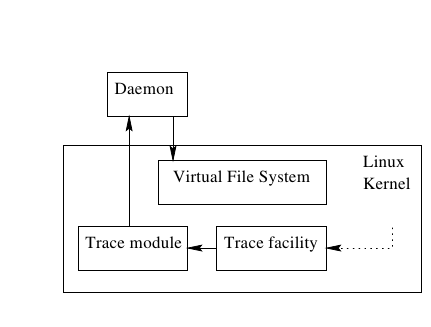
\includegraphics[scale=0.7]{ltt_arch.png}
       \caption{Arquitectura do \textit{Linux Trace Toolkit} \cite{Yaghmour:2000:MCS:1267724.1267726}}
	\label{fig:ltt_arch}
\end{figure}

%\subparagraph{Linux Trace Toolkit Viewer - }\label{cap:lttv_overview}
O \textit{Linux Trace Toolkit Viewer (LTTV)} é um projecto desenvolvido em paralelo com o \textit{LTT} e \textit{LTTng}, de modo a criar uma análise visual dos dados recolhidos por estas aplicações.
Esta ferramenta possibilita igualmente visualizar o traço de execução, uma vez que os dados recolhidos contêm uma estampilha temporal, do momento em que foram obtidos.

\subsubsection{OProfile}\label{cap:Oprofile_overview}
O \textit{OProfile} é uma ferramenta de monitorização, que efectua um perfil de utilização dos recursos da máquina, utilizando para o efeito a técnica de amostragem.
Assim, o \textit{OProfile}, em vez de a cada evento utilizar uma função para obter os dados, apenas a utiliza decorridos um certo número de eventos.
O recurso a este critério permite ao \textit{OProfile} ser menos perturbador, uma vez que nem sempre é necessário o universo dos eventos que as ferramentas de monitorização capturam, mas tão somente uma amostra.
Deste modo ao utilizar a amostragem, o \textit{OProfile}, introduz um menor grau de perturbação no sistema\cite{Will:TuninProgrOProf}.
% ser menos perturbador do sistema.
% it uses data sampling ... the others don't

Esta ferramenta é composta por três componentes principais: o módulo no núcleo (\textit{oprofile driver}), o \textit{daemon}/processo em nível utilizador que recolhe os dados obtidos da monitorização pelo módulo do núcleo (\textit{opcontrol}) e o \textit{opreport} e \textit{opannotate} que permitem criar relatórios, tal como se pode constatar na figura \ref{fig:oprofile_arch}.

\begin{figure}[!htb]
       \centering
       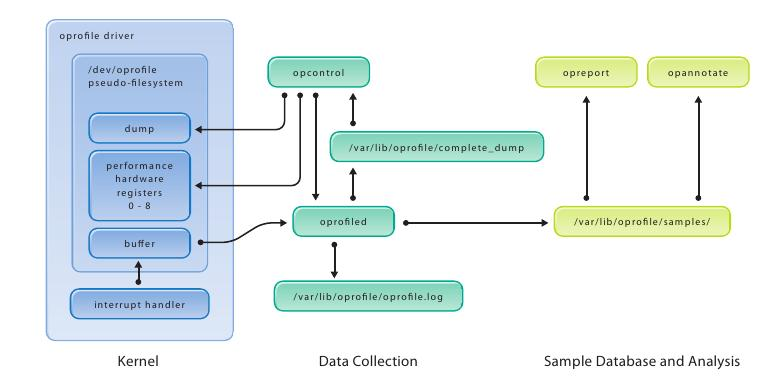
\includegraphics[scale=0.7]{oprofile_arch.jpg}
       \caption{Arquitectura do \textit{OProfile} \cite{Will:TuninProgrOProf}}
	\label{fig:oprofile_arch}
\end{figure}

O \textit{OProfile} não permite apenas efectuar o perfil de execução do núcleo \textit{Linux}, pode igualmente criar o perfil de execução dos processos de nível utilizador, que estão em execução na máquina.
Este perfil é criado com o auxílio do sistema de ficheiros virtual \textit{ProcFs}, que indica quais os processos em execução e respectivas zonas de memória utilizadas por estes.
O \textit{OProfile} regista os valores do \textit{program counter} (registo do processador que contém a próxima instrução a executar) e o instante em que este foi actualizado, assim com estes dados e conhecendo as zonas de memória, consegue identificar o processo em execução a cada amostragem.

%Para além de utilizar a técnica de amostragem, utiliza também \textit{buffers} especificos aos processadores, de modo a reduzir a sobrecarga exercida no sistema.

% outra abordagem 

\subsection{Suporte à monitorização}

Nas subsecções anteriores foram apresentadas ferramentas de monitorização e os seus mecanismos para efectuar a monitorização.
As ferramentas são importantes para efectuar análises aos dados obtidos.
Nas ferramentas, os diversos componentes que as constituem estão muito interligados, dificultando por vezes, o seu reaproveitamento e integração com outros componentes ou ferramentas.
Por outro lado, os mecanismos devem ser genéricos e independentes das ferramentas, para que estas possam ser desenvolvidas e os possam utilizar.
Como suporte à monitorização destacam-se o mecanismo \textit{KProbes} e a ferramenta \textit{Linux Kernel Stace Tracer}.
Em ambos é possível definir novos pontos, funções ou eventos a serem monitorizados, para além das funcionalidades já existentes nestas ferramentas.

\subsubsection{KProbes}\label{sect:KProbes_overview}

O \textit{KProbes} é um mecanismo de instrumentação dinâmica do núcleo do \textit{Linux}.
A \textit{API} permite que ferramentas, como o \textit{DProbes} ou o \textit{SystemTap} possam aceder às suas funcionalidades.
Esta encontra-se na versão principal do núcleo do sistema \textit{Linux}, desde a versão 2.6.9, o que indica tratar-se de um mecanismo bastante estável~\cite{kernel_debug_printk_on_fly,KProbesSite}.

O \textit{KProbes} utiliza a técnica do trampolim~\cite{Hollingsworth94dynamicprogram}, combinada com funções de \textit{handler} que efectuam as análises definidas pelo administrador.

Utilizando o \textit{KProbes} são possíveis três tipos de instrumentação: o \textit{KProbe}, o \textit{JProbe} e o \textit{KRetProbe}.
Cada um destes três tipos é específico de uma determinada funcionalidade.

\begin{itemize}
 \item \textbf{KProbe - } Utilizando o \textit{KProbe} pode detectar-se a execução de uma instrução, sendo esta indicada pela distância relativamente ao inicio de uma função instrumentada.
A indicação da função a instrumentar, pode ser definida recorrendo ao seu nome, ou ao seu endereço de memória.

\item \textbf{JProbe - } Um \textit{JProbe} destina-se a analisar os parâmetros, da função a instrumentar.
Quando é declarado um \textit{JProbe}, a função de \textit{handler} dessa chamada, tem de conter os mesmos tipos de argumentos que a função instrumentada, de forma a receber uma cópia destes.
 
 \item \textbf{KRetProbe - } Este tipo de análise tem como objectivo obter o valor de retorno da função que se pretende analisar.

\end{itemize}

\begin{figure}[!htb]
       \centering
       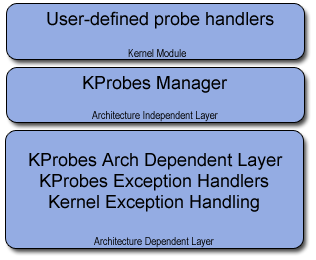
\includegraphics[scale=0.75]{KProbesArchitecture.jpg}
       \caption{Arquitectura do \textit{Kprobes} \cite{KProbesLwn}}
	\label{fig:kprobes_arch}
\end{figure}

\begin{figure}[!htb]
       \centering
       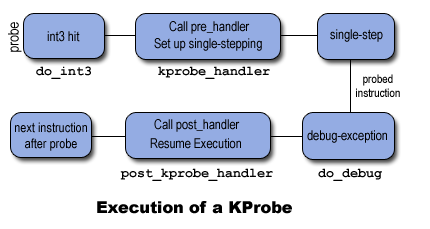
\includegraphics[scale=1.0]{KProbeExecution.png}
       \caption{Execução de um \textit{KProbe} \cite{KProbesLwn}}
	\label{fig:kprobe_execution}
\end{figure}

Para se obterem informações sobre as funções ou instruções que estão a ser monitorizadas, o \textit{KProbes} disponibiliza-as através de um ficheiro no \textit{DebugFs}.
Para utilizar o \textit{KProbes} é necessário criar um módulo para o núcleo do sistema de operação, com informações relativas às rotinas a instrumentar.
Para além destas, o módulo tem de conter igualmente os \textit{handlers} de análise, assim como outros parâmetros necessários à realização da instrumentação.

Quando o módulo é inserido no núcleo de sistema, o registo dos \textit{handlers} das funções a serem instrumentadas é efectuado de forma atómica.
A execução do \textit{KProbes} não utiliza nenhum \textit{mutex} ou outra forma de controlo de concorrência, apenas funciona com a preempção desligada.
Dependendo do contexto, os \textit{handlers} podem ser executados com as interrupções desligadas.

A instrumentação, pode processar-se copiando a instrução que se quer analisar para uma zona de memória, e substituindo essa instrução no código por uma interrupção (\textit{int3}).

Quando possível, o \textit{KProbes} utiliza instruções do processador, especializadas na depuração, de modo a minimizar o grau de perturbação.
A utilização da instrução \textit{int3} tem problemas de desempenho associados, por isso foi desenvolvido um modo alternativo para efectuar a instrumentação.
Este consiste na utilização de um \textit{jmp} incondicional, desta forma é possível obter um desempenho superior à utilização da instrução \textit{int3}.
Apesar de poder ser aplicado em diversas situações, não o pode ser em instruções que dependam do registo do processador \textit{eip} ou \textit{rip}, pois estas não podem usufruir desta optimização.

Apesar de ser possível instrumentar praticamente todo o núcleo do sistema de operação, existem algumas situações que podem requerer alguma perícia na forma como são tratadas.
Quando o compilador realiza substituição de funções por código \textit{inline}, as instruções que anteriormente estavam dentro da função passam a integrar o ponto onde foram substituídas, deixando de existir o ponto de entrada na função.
Assim sendo, a função deixa de existir, impossibilitando a instrumentação destas funções.
Não existe a possibilidade de instrumentar recursivamente uma função, ou seja, se uma função está a ser instrumentada e nas funções de \textit{handler} essa função é chamada, o \textit{KProbes} detecta que já está em execução e não permite que seja novamente interrompido, incrementando uma variável que indica que existiu um \textit{miss}.

Como anteriormente referido, este mecanismo de instrumentação do núcleo é utilizado por diversas ferramentas, de modo a instrumentar dinamicamente o código pertencente ao núcleo.
Duas das ferramentas que tiram partido deste mecanismo são o \textit{DProbes} e o \textit{SystemTap}.

\subsubsection{DProbes}
O \textit{DProbes} utiliza o \textit{KProbes} como suporte para efectuar a instrumentação dinâmica do núcleo de sistema.
Como a criação de pontos de análise são descrito em linguagem C ou \textit{assembly}, foi desenvolvida uma linguagem de mais alto nível de forma a simplificar a utilização desta aplicação.

Após se obterem os dados, estes podem ser transferidos para um ficheiro, para o \textit{daemon de logging} do núcleo de sistema, ou para uma porta série.
Existe, igualmente, a opção de interoperabilidade com o \textit{Linux Trace Toolkit}\cite{DProbes}.

%\subsubsection{SystemTap}\label{cap:Systemtap_overview}
\subsubsection{SystemTap}
O \textit{SystemTap} é uma ferramenta que possibilita o desenvolvimento mais fácil de módulos para o \textit{KProbes}, utilizando uma linguagem específica, de forma a ser segura e fácil de trabalhar.
Uma vez que os dados gerados estão no espaço de endereçamento de memória do núcleo, e o programa que os analisará se situa no espaço de endereçamento do utilizador, é necessário efectuar uma transferência de dados de um espaço para o outro.
O \textit{SystemTap} efectua esta transferência, recorrendo à utilização do sistema de ficheiros \textit{ReplayFs}, onde é possível escrever de forma rápida, sem comprometer a segurança do sistema\cite{Donovan2007,Jones2009}.

Apesar de no conjunto de aplicações desta ferramenta, existir um visualizador gráfico de dados recolhidos pelo \textit{SystemTap}, este só consegue analisar os \textit{TapSets} pré-definidos no \textit{SystemTap}.
Para ultrapassar esta limitação, novas ferramentas foram desenvolvidas.
Uma destas ferramentas designada por \textit{bootlimn}, está actualmente a ser desenvolvida no \textit{Google Summer of Code}, com o objectivo de utilizar o \textit{SystemTap} para recolher informações sobre o arranque do sistema, agregando estes dados no formato \textit{XML}.
Os dados recolhidos, permitem visualizações gráficas do processo de inicialização do sistema, bem como da utilização de disco e \textit{CPU}.
Outro projecto conhecido como \textit{Systemtap GUI}, engloba o \textit{System Tap Editor Plug-in} para a ferramenta \textit{Eclipse}, sendo um ambiente onde podem ser analisados e visualizados os dados recolhidos pelo \textit{SystemTap} a partir do \textit{Eclipse}.

%O \textit{SystemTap} actualmente está a ser desenvolvido por empresas de reconhecido mérito internacional, nomeadamente a \textit{Red Hat}, a \textit{IBM}, a \textit{Hitachi} e a \textit{Oracle}.




%\subsubsection{DProbes}\label{cap:Dprobe_overview}

\subsubsection{Linux Kernel State Tracer}
% Linux Kernel State Tracer(LKST) records information as trace data about events in the Linux Kernel. It records various events like process context switch, send signal, exception, memory allocation, send packet, and so on. 

O \textit{Linux Kernel State Tracer(LKST)} obtém informações referentes ao núcleo de sistema, de forma a criar um traço de execução, e consegue capturar diferentes eventos como trocas de contexto, envio de sinais, alocação de memória, transmissão de pacotes, etc.

% a\subparagraph{DJProbe}
\label{cap:djprobe}
  % Este sistema é mais leve devido à forma como é feito o ``trap'' pois não usa o int 3
% Duvidas na forma como é controlado o sistema na presença de processadores maquinas com multiplos processadores.
% Não utiliza o int 3 para fazer o trap por isso segundo o artigo fica mais leve que o KProbe e o JProbe.
% DJProbe  quer dizer Direct Jump Probe faz um jmp e não usa o int 3.
Actualmente, está a ser desenvolvido um subprojecto do \textit{Linux Kernel Stace Tracer} designado por \textit{Direct Jump Probe}.
O \textit{Direct Jump Probe} é uma optimização à utilização do \textit{trap int3}, presente em alguns processadores, e que pode trabalhar em conjunto com o \textit{KProbes}.
Esta optimização pode ser verificada no relatório\cite{Hiramatsu2005}.


\subsection{Comparação entre os diferentes sistemas de instrumentação dinâmicos}
% \todo{completar esta tabela}
\begin{table}[h!]
\begin{center}
\caption{Tabela Comparativa dos sistemas de instrumentação}
\label{tab:inst_compare}
\begin{tabular}{|l||c|c|c|}
\hline
Instrumentação & Amostragem / Traço & Análise de Parâmetros & Deamon \\
\hline
KProbes & Traço & Permite & Não necessita \\
\hline
LKST & Traço & Permite & Necessita \\
\hline
LTT & Traço & Não permite & Necessita \\
\hline
OProfile & Amostragem & Não permite & Necessita \\
\hline

\end{tabular}
\end{center}
\end{table}

%Da observação da tabela \ref{tab:inst_compare} pode inferir-se que: ToDo

A tabela \ref{tab:inst_compare} permite fazer uma comparação entre algumas das caracteristicas destes sistemas de instrumentação presentes no núcleo de sistema do \textit{Linux}, segundo os seguintes critérios: metodologia da captura (por traço ou por amostragem), análise dos parâmetros das funções instrumentadas e a necessidade de ter um \textit{deamon} para a recolha de dados provenientes do sistema de monitorização.
Se a necessidade de ter um \textit{deamon} a executar de forma a coligir e organizar os dados, pode penalizar o desempenho do sistema, a possibilidade de analisar os parâmetros das funções instrumentadas é um ponto a favor dos sistemas \textit{KProbes} e do \textit{LKST}.



\section{Transferência de dados}
\label{sect:kernel_user_comm}


Quando se recorre a alguma fonte para a obtenção de dados, é necessário que estes sejam transferidos para o sistema que os quer consultar.
Assim, os dados que foram obtidos no núcleo têm de ser transferidos para as outras componentes ou para os processos que os requereram.

No intuíto de melhorar a partilha de recursos externos, o controlo dá-se ao nível do núcleo do sistema, pelo que parte das comunicações dos utilizadores com dispositivos externos, é efectuada através do núcleo de sistema.
Não sendo apenas exclusivo dos recursos externos, recursos que sejam partilhados por mais que um processo, em geral são partilhados e controlados através do núcleo.
Desta forma é necessário existirem modos de comunicação / transferência de dados dentro do núcleo e, entre este e os processos.

%Incluir por aqui a informação de mmaps, ring buffers e afins ....
% colocar a parte interna e verificar o mmap que tb faz parte do utilizador
% verificar o mmap da parte de utilizador
%texto explicativo de interno e externo 
\subsection{Técnicas de transferência de dados}

Devido há necessidade de transferir informações entre diferentes \textit{buffers} dentro do núcleo de sistema, foram desenvolvidas técnicas tendo sempre como referência a minimização da sobrecarga.
De entre as diferentes técnicas de transferência interna de informação ao núcleo do sistema, merecem especial relevo:

\paragraph*{\textit{MMAP} - }

Esta técnica que é implementada utilizando páginas de memória partilhadas, reduzindo as transferências e gastos de memória, proporciona a possibilidade de mapear um canal para memória potenciando assim, a partilha de dados não só entre diferentes processos como igualmente entre os processos e o núcleo, que necessitem de aceder aos dados do mesmo canal.
A partilha de dados de \textit{IO} é uma vertente que tem sido objecto de desenvolvimento, de forma a aumentar o desempenho, porquanto permite a partilha de dados entre um ou mais programas, e o núcleo de operação.
Esta partilha evita a necessidade de copiar dados dos espaços de endereçamento do núcleo para o do utilizador e vice versa.

\paragraph*{Zero Copy - }

Esta técnica de transferência de dados sem que existam cópias dos \textit{buffers} pertencentes ao núcleo de sistema e ao espaço de utilizador, permite que os dados sejam partilhados por diferentes entidades, sem necessidade de criação de novos \textit{buffers} e cópias de dados, uma vez que apenas são passadas as referências.

\paragraph*{Ring Buffers - }

Esta técnica consiste num aproveitamento dos recursos partilhados já alocados, mas que se tornaram desnecessários, estando desta forma disponíveis para nova utilização.
Os \textit{Ring Buffers} são utilizados tendo presente a relação custo / benefício, isto é, quando o peso da criação e destruição de elementos é comparativamente superior à reutilização dos recursos já alocados.
É igualmente utilizada em situações de \textit{"produtor-consumidor"}, ou seja, quando é necessário manter a ordem dos elementos.


\subsection{Interface do sistema com os processos}
% {\color{red}
% \paragraph*{}
% INDICAR QUAIS OS SISTEMAS QUE OS UTILIZAM
% 
% DISTINÇÂO ENTRE OS DIFERENTES SISTEMAS
% }

Devido à necessidade de análise de estruturas e dados do núcleo de sistema, e de oferecer uma interface familiar baseada nos sistemas de ficheiros, foram criados diferentes subsistemas com vista à sua satisfação.
Um destes subsistemas é o \textit{ProcFs}, que existe no núcleo de sistema do \textit{Linux} desde as primeiras versões.
Outros como o \textit{DebugFs} ou o \textit{RelayFs} são mais recentes e com novas abordagens.
%diferentes abordagens e o pq de ter de existirem estas formas

\paragraph*{}
De forma a obter informações relativas a estruturas dentro do núcleo de sistema, foram referenciados os seguintes sistemas de comunicação entre o utilizador e o núcleo:

\paragraph*{ProcFs - }\label{cap:ProcFs_overview}

Desenvolvido para obter informações relativas aos processos, tem sido utilizado desde as primeiras versões do núcleo de sistema do \textit{Linux}.
Apesar de novos sistemas como o \textit{SysFs} terem sido criados, continua a ser extensivamente utilizado pelas aplicações, pois este contém informações disponíveis para o nível utilizador sobre estruturas e dados dos processos localizadas no núcleo.
Esta é uma das \textit{API's} de comunicação, entre o núcleo e as aplicações, mais utilizadas, não obstante ter crescido de forma desorganizada.

\paragraph*{SysFs - }\label{cap:SysFs_overview}

Este sistema de ficheiros virtual foi desenvolvido para colmatar algumas deficiências encontradas no \textit{ProcFs}.
Estes problemas situam-se basicamente na forma desorganizada como a quantidade de informação disponibilizada está distribuída sobre o \textit{ProcFs}.
Este novo sistema de ficheiros virtual, evidencia restrições na disponibilização das informações, uma vez que apenas é possível visualizar e modificar um \textit{KObject} por ficheiro, assim é possível efectuar uma normalização da apresentação das estruturas do núcleo.
Esta limitação conduziu a que outros sistemas de ficheiros virtuais, nomeadamente o \textit{DebugFs} e o \textit{RelayFs}, fizessem a sua aparição com vista a colmatar esta situação.

\paragraph*{DebugFs - }\label{cap:DebugFs_overview}

Este sistema foi essencialmente criado para ultrapassar as dificuldades sentidas pelos programadores, na utilização de um sistema de ficheiros tão restritivo como o \textit{SysFs}.
Apesar de já existirem dois sistemas de ficheiros virtuais, o \textit{ProcFs} e o \textit{SysFs}, este tentou colmatar os problemas que se apresentavam, não obstante não se mostrar tão estruturado como o \textit{SysFs}, tem melhor organização de dados que o \textit{ProcFs}.

O sistema de instrumentação do núcleo de sistema \textit{Linux}, \textit{KProbes}, utiliza este sistema de ficheiros virtual, de forma a apresentar os pontos onde existe instrumentação no núcleo de sistema.

\paragraph*{RelayFs - }\label{cap:RelayFs_overview}

Este sistema de ficheiros virtual foi desenvolvido tendo em mente a transferência de grandes quantidades de dados entre o núcleo de sistema e o espaço de utilizador.
O \textit{RelayFs} responde a esta exigência, fazendo uso de novas primitivas onde são mais reduzidas as zonas de controlo de concorrência~\cite{Donovan2007,To03relayfs:an}.

\paragraph*{NetLink - }\label{cap:NetLink_overview}
O \textit{NetLink} utiliza um método de comunicação baseado em \textit{sockets}, para estabelecer a comunicação entre o núcleo de sistema e os processos, em nível utilizador. 
 Tendo como abstracção os \textit{sockets}, este sistema tem igualmente a possibilidade de enviar dados para múltiplos processos, devido à utilização das primitivas de envio colectivo (\textit{Multicast}).
% \todo{Explicar melhor o NetLink}
 É com base no \textit{NetLink}, que a comunicação entre processos dentro da mesma máquina (\textit{IPC}) é implementada.
%Isto ja e novo
 A comunicação com diferentes partes do subsistema de rede é efectuada recorrendo a este sistema de \textit{sockets}.


\subsection{Comparação entre sistemas de transferência de dados}

\paragraph*{}
Como se pode verificar através da tabela \ref{tab:transf_compare}, que compara a estruturação dos dados de cada Sistema, com o volume de dados que é possível com facilidade transferir, o \textit{RelayFs} e o \textit{NetLink} são os dois sistemas de comunicação que, não tendo estruturação fixa dos dados, conseguem transferir um volume superior de dados, comparativamente com os restantes objecto da análise.
%Se limitarmos a análise comparativa aos sistemas \textit{RelayFs} e \textit{NetLink}, constatamos que o volume de dados que é possível transferir pelo primeiro é superior ao verificado no \textit{NetLink}.

% \todo{Corrigir esta tabela}
\begin{table}[!htbp]
\begin{center}
\caption{Tabela Comparativa de transferência de dados entre processos e núcleo de sistema}
\begin{tabular}{|l||c|c|}
\hline
Sistema & Estruturação de Dados & Volume de dados \\
\hline
ProcFs & Com & Reduzido \\
\hline
SysFs & Com & Reduzido \\
\hline
DebugFs & Com & Reduzido \\
\hline
RelayFs & Sem & Bastante Elevado \\
\hline
NetLink & Sem & Elevado \\
\hline
\end{tabular}

\label{tab:transf_compare}
\end{center}
\end{table}
 
\section{Captura de tráfego de um processo específico}
\label{sect:outras_abordagens}

A captura do tráfego, respeitante a um processo genérico, foi alvo de estudo em \cite{1688981} e em \cite{duarte10,Farruca:2009}, esta última, uma dissertação de mestrado.

No primeiro trabalho, foi desenvolvido um sistema de captura de pacotes de um determinado processo, utilizando um módulo no núcleo de sistema que intercepta e captura os pacotes do processo.

Este sistema é constituido por três componentes essenciais: um dentro do núcleo de sistema e dois em nível utilizador.
Na realização do trabalho, foi utilizada a ferramenta \textit{KProbes} para a monitorização de algumas funções do núcleo de sistema \textit{Linux}, de forma a conhecer quais os portos que vão ser utilizados por uma determinada aplicação.
Logo que obtida, a informação é enviada para um processo em nível utilizador que tem o registo de todos os portos que estão a ser utilizados pela aplicação objecto de monitorização.
Se esse porto não estiver a ser monitorizado, essa informação é passada a outro processo que utiliza a biblioteca \textit{PCap} de forma a capturar o tráfego existente nesse porto.


\begin{figure}[h!]
       \centering
       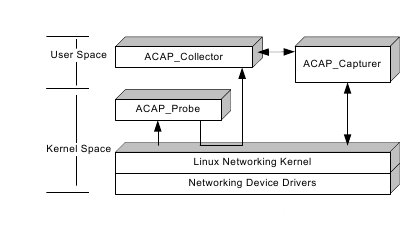
\includegraphics[height=2in]{captura_kprobes_paper}
       \caption{Arquitectura da monitorização de tráfego \cite{1688981}}
	\label{fig:paper_capture_kprobes}
\end{figure}


Analisando a arquitectura de monitorização de tráfego representada na figura~\ref{fig:paper_capture_kprobes}, o ACAP\_Collector e o ACAP\_Capturer, estão em nível utilizador, de onde se infere que o desempenho desta ferramenta sofre com as trocas de contexto e alterações da captura efectuada no \textit{PCap}.

Relativamente ao segundo trabalho, foram implementadas duas abordagens: uma com monitorização da aplicação e outra através de informações pertencentes ao núcleo do sistema de operação.
No que à primeira diz respeito, a monitorização efectuada processou-se através da interceptação das chamadas à bibiloteca \textit{LibC}, para a utilização de \textit{sockets}, criando uma bibiloteca partilhada com a mesma sintaxe das chamadas que são utilizadas.
A opção pela utilização deste método, implica definir a variável de ambiente \textit{LD\_PRELOAD}, de forma a operar esta intercepção.
Como esta biblioteca está em nível utilizador, mostra-se necessário capturar todos os pacotes e apenas em nível utilizador visualizar o tráfego respeitante ao processo.
Esta obrigatoriedade, de capturar todos os pacotes, pode constituir uma tarefa com elevado grau de perturbação do sistema.

No que à segunda abordagem se refere, o método de monitorização utilizado baseou-se na consulta efectuada de forma regular com intervalos reduzidos, dos dados referentes aos portos de comunicação, utilizados pela aplicação, que são exportados pelo núcleo através do \textit{ProcFs}.
Esta forma de monitorização consome demasiados recursos e não se mostra totalmente fiável, na medida em que quanto menor o intervalo de tempo utilizado, maior é a perturbação apresentada pelo sistema.

O dinamismo das aplicações, nomeadamente das aplicações multimédia, deu origem a diversos estudos sobre a forma de monitorização de rede, que estas necessitam.
Estas aplicações utilizam diversos fluxos de dados, designadamente de transmissão e de recepção.
Em geral, as aplicações multimédia, com base na \textit{internet} utilizam uma metodologia cliente/servidor, onde o servidor aguarda pedidos do cliente num determinado porto.
O cliente, conhecendo antecipadamente este porto, liga-se.
A partir deste ponto, iniciam-se trocas de informações, que irão originar a troca de portos dinâmicos e posteriormente o processo de transmissão/recepção de dados multimédia.

As aplicações multimédia assentes na \textit{Internet} são, apenas, um exemplo de aplicações com diversos fluxos, em que as portas de comunicação entre as aplicações, são negociadas dinamicamente.

Como o referido em \ref{sect:LibPcap}, a captura de pacotes é definida em filtros estáticos e para capturar este tipo de tráfego, é necessário conhecer esses protocolos e depois modificar os filtros definidos, de modo a acompanhar o protocolo.
Esta forma de captura mostra-se bastante ineficaz, o que motivou a que fossem estudadas algumas alternativas, tendo em vista a correcção desta situação.
Os projectos \textit{mmdump}\cite{505678}, %\textit{Fairly Fast Packet Filters (FFPF)}\cite{1251278} 
e \textit{Swift}\cite{1387609} são dois destes casos estudados, que merecem especial relevância e que adiante se analisam:

\paragraph*{MMDump - } É uma ferramenta de monitorização de protocolos multimédia com suporte na rede.
Esta aplicação tem como base o \textit{tcpdump}, sendo a captura de pacotes efectuada através da utilização de filtros.
Para determinar os portos a obter, é necessário analisar o conteúdo dos pacotes direccionados a portos específicos e, a partir destes é possível identificar os novos portos negociados dinamicamente pela aplicação, para proceder à alteração dos filtros a aplicar.
Como a alteração, que é constituída pela cópia do novo filtro para o núcleo e verificação de segurança, de forma a validá-lo, é um processo demorado, é necessário reduzir este tempo, com o objectivo de ter uma aplicação que consiga minimizar o grau de perturbação no sistema.

Na alteração do filtro, foi verificado que existe um certo padrão, que consiste em pré-estabelecer uma parte comum a ser adicionada ao filtro, e apenas alterar a parte referente aos portos.

Esta forma de monitorização é muito específica, pelo que é imprescindível reconhecer todo o protocolo interno de comunicação.
Assim, para cada novo protocolo a monitorizar, é necessário acrescentar um novo módulo com a interpretação desse protocolo.

% \paragraph*{\textit{Fairly Fast Packet Filter} (FFPF)}

\paragraph*{\textit{Swift} - }
É uma ferramenta de criação de filtros, cujo principal objectivo é a melhorar o desempenho da utilização destes, na captura do tráfego de rede.
Nesta ferramenta, foi avaliado o tempo necessário para a alteração dos filtros utilizando o \textit{Linux Socket Filtering}, pois estes são os filtros de referência no sistema de operação \textit{Linux}.
A aplicação destes filtros a partir da biblioteca \textit{PCap} compreende três fases: cópia do filtro definido em nível utilizador para o núcleo de sistema, verificação de segurança, e aplicação do filtro.
De forma a diminuir a latência de actualização dos filtros, foi criada uma especificação de modo a que estes não necessitassem de ser analisados relativamente à segurança, visto que a própria linguagem garante as propriedades de segurança necessárias.
Com este novo \textit{instruction set} e, sem necessidade de verificação, foi reduzida a latência de actualização dos filtros, o que conduziu a um aumento de desempenho na utilização de filtros dinâmicos.


%\section{Conclusão}





%\section{Filtragem de pacotes de um processo através do \textit{Netfilter}}

%O \textit{NetFilter} é o sistema de filtragem de pacotes do núcleo do \textit{Linux} que irá ser apresentado na secção \ref{}.
%Foi implementado um módulo no núcleo utilizando o \textit{NetFilter} que filtra os pacotes pertencentes a um processo ou utilizador.
%Este sistema, verifica relativamente a cada pacote que é recebido ou enviado, se este faz parte do processo ou processos pertencentes a um utilizador, verificando canal a canal se o identificador do canal do pacote é igual ao canal do processo.


%Falta falar do ipt\_owner do iptables entre outros ....

\section{Conclusão}
\label{sec:segundo:conclusion}
Como se pode observar neste capítulo, existe a possibilidade de melhorar a monitorização de rede do \textit{Linux}.
O mecanismo de instrumentação genérico do \textit{Linux}, \textit{KProbes}, permite que se efectuem análises no núcleo de modo generalista, o que para obter as interacções dos processos com as interfaces de rede sem que se assista à instrumentação do código dos processos e com baixa sobrecarga será um mecanismo de instrumentação dinâmico a ter em conta para o desenvolvimento de um mecanismo de monitorização genérico de rede de um processo.

Por forma evitar a sobrecarga da transferência de dados irrelevantes para nível utilizador, pretende-se estender a captura com filtros do \textit{LSF}, para que passe a ter em conta os estado do processo alvo obtido pela instrumentação anterior.
Ao efectuar este processamento no núcleo, não se incorre na reinicialização de todo o mecanismo de captura do \textit{PCap}, salvaguardando a perda de pacotes relevantes e diminuindo a sobrecarga introduzida.
